%!TEX root = ../thesis.tex

\section{関連研究}
歩行者の複雑な動きを予測するために,深層学習を応用しようという研究が,近年注目を集めている.
深層学習を歩行者の軌道予測に応用した例として,Alexandreら\cite{s-lstm}は,人間の動きを学習し,未来の軌跡を予測できるLSTMモデルを提案している.この研究は,歩行者の軌道予測に着目した最も初期の深層学習モデルの一つである.Social-LSTMは,\figref{Fig:s-lstm}のように各軌跡に1つのLSTMを使用し,プーリング機構を用いて,LSTM間で情報を共有している.このシステムにより,複数の個人にわたって相互作用から生じるさまざまな非線形行動をうまく予測することに成功した.

\begin{figure}[hbtp]
     \centering
    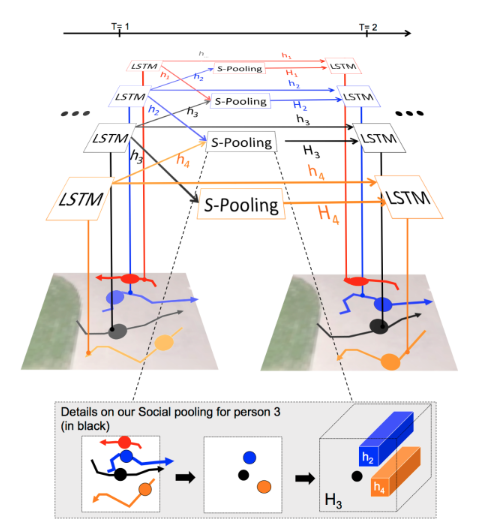
\includegraphics[keepaspectratio, scale=0.56]
         {images/s-lstm.png}
    \caption{Overview of Social-LSTM method.\protect\footnotemark[1]}
    \label{Fig:s-lstm}
\end{figure}

\protect\footnotetext[1]{\cite{s-lstm}より引用}

Zhangら\cite{sr-lstm}は,LSTMのシーケンス学習能力にエージェント間の相互作用をモデル化するため,\figref{Fig:sr-lstm-str}のようなLSTMネットワークの情報精密化モジュールを提案している.この研究では,\figref{Fig:sr-lstm}のようにAttentionメカニズムにより,各歩行者の他者への影響を重み付けしている.

% \vspace{0.8zh}

\begin{figure}[hbtp]
     \centering
    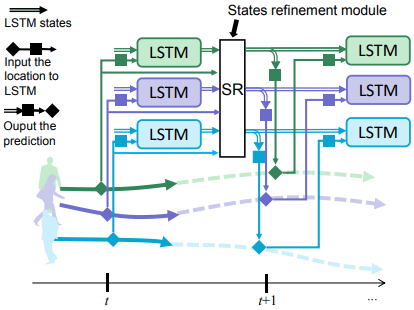
\includegraphics[keepaspectratio, scale=0.65]
         {images/sr-lstm-str.png}
    \caption{Framework overview of proposed SR-LSTM.\protect\footnotemark[2]}
    \label{Fig:sr-lstm-str}
\end{figure}

\begin{figure}[hbtp]
     \centering
    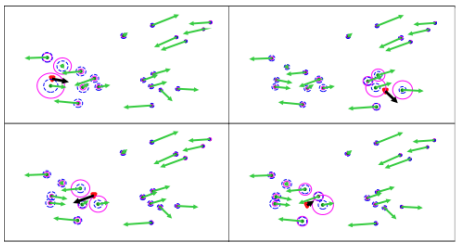
\includegraphics[keepaspectratio, scale=0.65]
         {images/sr-lstm.png}
    \caption{Illustration of the pedestrian-wise attention.\protect\footnotemark[2]}
    \label{Fig:sr-lstm}
\end{figure}

\protect\footnotetext[2]{\cite{sr-lstm}より引用}

同様に,歩行者の注意に着目した研究をKosarajuら\cite{s-bigat}も行っている.この研究は,LSTMを用いて各歩行者の軌跡をモデル化し,グラフアテンションネットワーク(GAT)を用いて,現実的な歩行者の軌道予測を実現している.この研究では,グラフは\figref{Fig:s-bigat}のように,歩行者をノード,距離をエッジとしてモデル化される.このグラフ構造を用いることで,歩行者間の相互作用を効果的に捉え,より正確な軌道予測が可能となる.

\begin{figure}[hbtp]
     \centering
    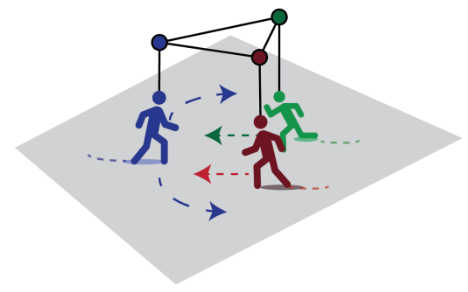
\includegraphics[keepaspectratio, scale=0.4]
         {images/s-bigat.png}
    \caption{Illustration of the pedestrian-wise attention.\protect\footnotemark[3]}
    \label{Fig:s-bigat}
\end{figure}

\protect\footnotetext[3]{\cite{s-bigat}より引用}

また,Mohanmedら\cite{s-stgcnn}は軌跡をグラフとしてモデル化し,歩行者間のユークリッド距離で重み付けされたエッジは歩行者間の相互作用を表している.\figref{Fig:s-stgcnn}のように,モデルはグラフ畳み込みニューラルネットワークと時間畳み込みネットワーク(TCN)を用いて,時空間グラフ上で動作し,一度にシーケンス全体を予測できるようにしている.

\begin{figure}[hbtp]
     \centering
    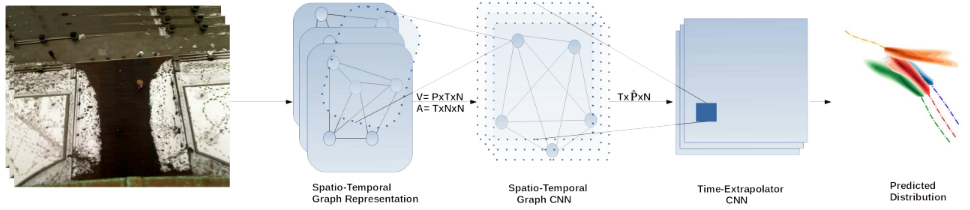
\includegraphics[keepaspectratio, scale=0.39]
         {images/s-stgcnn.png}
    \caption{The Social-STGCNN Model.\protect\footnotemark[4]}
    \label{Fig:s-stgcnn}
\end{figure}

\protect\footnotetext[4]{\cite{s-stgcnn}より引用}

\newpage

移動ロボットで歩行者の軌道予測を行う場合,歩行者同士の相互作用の他にロボットと人間にも相互作用が存在する.そのため,歩行者だけでなく,ロボットの行動も考慮した軌道予測が必要である.

丹野ら\cite{si2023-tanno}は,歩行者の軌道予測に過去の動きだけでなく,\figref{chap:element_technology}のように,ロボットが選択する将来の動きを考慮して予測をしている.実験では,ロボットの将来の行動を考慮しない場合と比較して,ロボットの動きに合わせて変化する歩行者の動きを予測できることが確認されている.しかし,学習器の事前学習でデータセット内の人間をロボットと見なして学習している.つまり,歩行者の行動を移動ロボットの行動に近似できるという前提の上で学習している.それならば,モデル構造のエンコード部分を除外し,ネットワークを人間とロボットで共有化させることができる可能性がある.これは,ネットワークの肥大化を防いだり,学習の手間を低減させるねらいがある.4章では,この論文を参考に実験を行う.

% 丹野ら\cite{future-robot}は,歩行者の軌道予測に過去の動きだけでなく,\figref{chap:element_technology}のように,ロボットが選択する将来の動きを考慮して予測をしている.実験では,ロボットの将来の行動を考慮しない場合と比較して,ロボットの動きに合わせて変化する歩行者の動きを予測できることが確認されている.

\begin{figure}[hbtp]
     \centering
    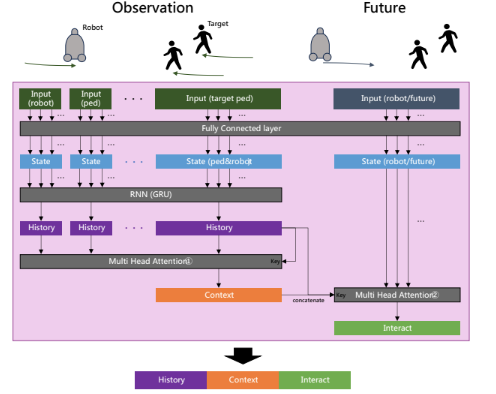
\includegraphics[keepaspectratio, scale=0.70]
         {images/future-robot.png}
    \caption{Encoder structure.\protect\footnotemark[5]}
    \label{Fig:future-robot}
\end{figure}

\protect\footnotetext[5]{\cite{si2023-tanno}より引用}

このように,深層学習を歩行者の軌道予測タスクに応用する例は少なくない.しかし,その多くは学習器の訓練を鳥瞰図のデータセットを用いて行っている.それに伴い,移動ロボットを対象にしたものが少ない.また,移動ロボットを対象している場合においても,予測対象にトラッキングセンサなどを取り付け,環境に介入している場合やシミュレータで予測対象の真値を取得しており,移動ロボットのセンシングしたデータだけで完結していないものが多い.そのため,深層学習を応用した歩行者の予測結果を移動ロボットのナビゲーションで利用しようとする研究例は現時点ではあまり報告されていない.

\newpage